\documentclass{standalone}
\usepackage[utf8]{inputenc}
\renewcommand*\familydefault\sfdefault

\title{CIS 114 Final Project Proposal - UML Use Case Diagram}
\author{Leomar Durán}
\date{27 November 2021}

%%%%%%%%%%%%%%%%%%%%%%%%%%%%%%%%%%%%%%%%%%%%%%%%%%%%%%%%%%%%%%%
% CHANGELOG :
%     2021-11-27t15:37
%         integrated all actor loops
%
%     2021-11-27t15:37
%         loop to place actors
%         better loop variables in \actor
%
%     2021-11-27t15:13
%         actor labels, associations in loop,
%         better loop variables in document
%
%     2021-11-27t03:45
%         detailed administrator, looped repetitive tasks
%
%     2021-11-27t03:15
%         associated user to their use cases
%
%     2021-11-27t03:08
%         add the user and first server actor
%
%     2021-11-27t01:24
%         create the package of use cases
%
%     2021-11-26t20:37
%         documented \actor[5][1]
%
%     2021-11-26t20:25
%         added ports to actor
%
%     2021-11-26t16:40
%         created actor shapes
%
%     2021-11-26t14:53
%         started with an empty node
%%%%%%%%%%%%%%%%%%%%%%%%%%%%%%%%%%%%%%%%%%%%%%%%%%%%%%%%%%%%%%%

\usepackage{tikz} % for tikzpicture
\usetikzlibrary{calc}
\usetikzlibrary{positioning}
\usetikzlibrary{matrix}
\usetikzlibrary{shapes}

% The actor shape without scope or ports
\newcommand*\unscopedactor{%
    \draw (0,22.5pt) circle (7.5pt);% head
    \draw (0,15pt) -- ++(0,-25pt) -- ++(-15pt,-20pt);% body and left leg
    \draw (-15pt,10pt) -- ++(30pt,0);% arms
    \draw (0,-10pt) -- ++(15pt,-20pt)% right leg
}%

% The actor shape including scope and ports
% @param * adds the last x/y-coordinates to x/y-shifts
% @param 1 scale (default 1)
% @param 2 port name prefix
% @param 3 x-shift
% @param 4 y-shift
% @param 5 extensions after the actor within scope
\makeatletter
    \newcommand*\actor{%
        \@ifstar%
            \actor@star%
            \actor@nostar%
    }%
    \newcommand*\actor@star[5][1]{%
        % coordinates stored for positioning actors
        \newdimen\xcoord
        \newdimen\ycoord
        \pgfgetlastxy\xcoord\ycoord;%
        \actor@nostar[#1]{#2}{\xcoord+#3}{\ycoord+#4}{#5}%
    }%
    \newcommand*\actor@nostar[5][1]{%
        \begin{scope}[scale=#1,xshift=#3,yshift=#4,line width=1pt]%
            \unscopedactor;%
            % create the actor ports
            % \port actor port
            % \x/\y actor coordinates
            \foreach \port/\x/\y in {%
                /0/0,% central port
                -north/0/30pt,%
                -west/-15pt/10pt,%
                -east/15pt/10pt,%
                -south/0/-30pt%
            }%
                \coordinate (#2\port) at (\x,\y);%
            % \foreach \port/\x/\y
            #5%
        \end{scope}%
    }%
\makeatother

\def\echoeast{east}
\def\echowest{west}

\begin{document}

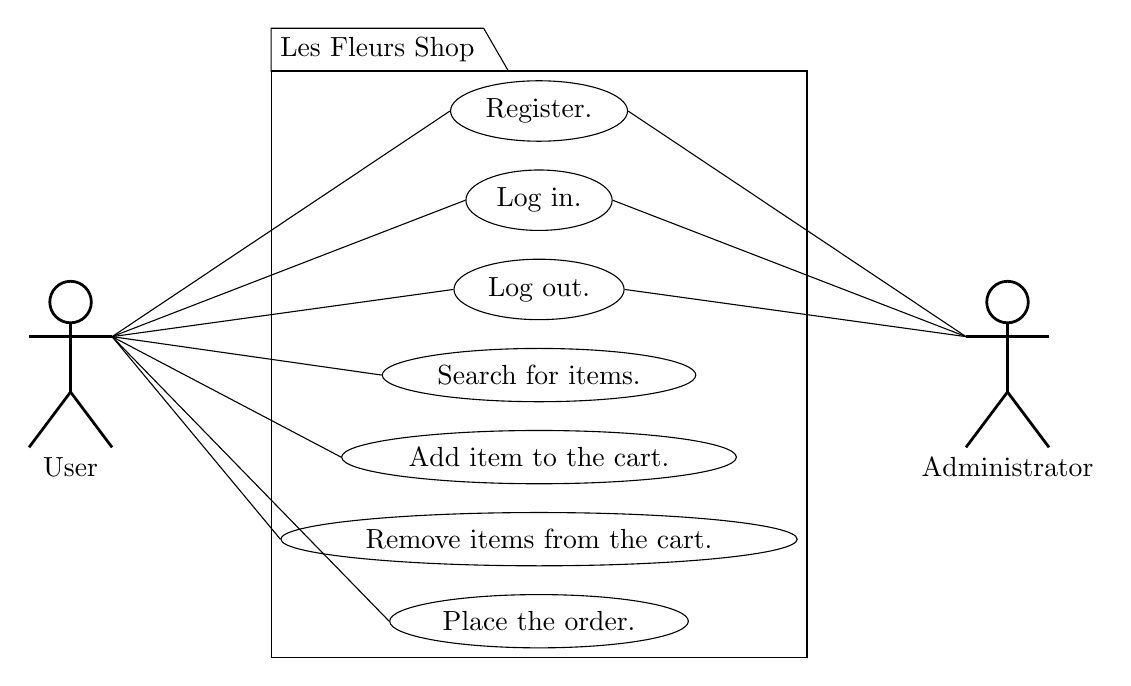
\begin{tikzpicture}
    [%
        package head/.style={%
            draw,%
            trapezium,%
            trapezium left angle=90,%
            anchor=bottom left corner,%
            yshift=-0.5pt%
        },%
        package body/.style={%
            draw,%
            matrix of nodes,%
            row sep=10pt,%
            every node/.style={use case},%
        },%
        use case/.style={%
            draw,%
            ellipse%
        }%
    ]%
%
    \matrix[package body] (les-fleurs-body) {
        Register.
    \\
        Log in.
    \\
        Log out.
    \\
        Search for items.
    \\
        Add item to the cart.
    \\
        Remove items from the cart.
    \\
        Place the order.
    \\
    };
    \node[package head] at (les-fleurs-body.north west) {Les Fleurs Shop};
    \foreach \side/\actorname/\x in {west/User/-1in,east/Administrator/1in} {
    }
%
    % draw each actor, its label and associations
    % \side the actor is of the use case packages
    % \Map actor--user case mappings
    \foreach \side/\Map in {%
        west/{%
            User/{1,2,...,7}%
        },%
        east/{%
            Administrator/{1,2,3}%
        }%
    }{
        % set according to \side
        %     \pactor port of actor from which to draw
        %     \actorx distance from the \side
        \ifx\side\echowest
            \def\pactor{east}
            \def\actorx{-1in}
        % \ifx\side\echowest
        \else\ifx\side\echoeast
            \def\pactor{west}
            \def\actorx{1in}
        \fi\fi % \side\echoeast
%
        % \actorname
        % \Usecases use case set
        \foreach \actorname/\Usecases in \Map {
% place the actor
            \node at (les-fleurs-body.\side) {};
            \actor*\actorname\actorx0;
% label the actor
            \node[below=0pt of \actorname-south] {\actorname};
% associations from the actor
            % \usecaseno use case number
            \foreach \usecaseno in \Usecases {
                \draw (\actorname-\pactor) -- (les-fleurs-body-\usecaseno-1.\side);
            } % \foreach \usecaseno
        } % \foreach \actorname/\Usercases
    } % \foreach \side/\Map
\end{tikzpicture}

\end{document}
